%%%%%%%%%%%%%%%%%%%%%%%%%%%%%%%%%%%%%%%%%
% Beamer Presentation
% LaTeX Template
% Version 1.0 (10/11/12)
%
% This template has been downloaded from:
% http://www.LaTeXTemplates.com
%
% License:
% CC BY-NC-SA 3.0 (http://creativecommons.org/licenses/by-nc-sa/3.0/)
%
%%%%%%%%%%%%%%%%%%%%%%%%%%%%%%%%%%%%%%%%%

%----------------------------------------------------------------------------------------
%	PACKAGES AND THEMES
%----------------------------------------------------------------------------------------

%%%%%%%%%%%%%%%%%%%%%%%%%%%%%%%%%%%%%%%%%
\documentclass{beamer}

\mode<presentation> {

% The Beamer class comes with a number of default slide themes
% which change the colors and layouts of slides. Below this is a list
% of all the themes, uncomment each in turn to see what they look like.

%\usetheme{default}
%\usetheme{AnnArbor}
%\usetheme{Antibes}
%\usetheme{Bergen}
%\usetheme{Berkeley}
%\usetheme{Berlin}
%\usetheme{Boadilla}
%\usetheme{CambridgeUS}
%\usetheme{Copenhagen}
%\usetheme{Darmstadt}
%\usetheme{Dresden}
%\usetheme{Frankfurt}
%\usetheme{Goettingen}
%\usetheme{Hannover}
%\usetheme{Ilmenau}
%\usetheme{JuanLesPins}
%\usetheme{Luebeck}
%\usetheme{Madrid}
%\usetheme{Malmoe}
%\usetheme{Marburg}
%\usetheme{Montpellier}
%\usetheme{PaloAlto}
%\usetheme{Pittsburgh}
%\usetheme{Rochester}
\usetheme{Singapore}
%\usetheme{Szeged}
%\usetheme{Warsaw}

% As well as themes, the Beamer class has a number of color themes
% for any slide theme. Uncomment each of these in turn to see how it
% changes the colors of your current slide theme.

%\usecolortheme{albatross}
%\usecolortheme{beaver}
%\usecolortheme{beetle}
%\usecolortheme{crane}
%\usecolortheme{dolphin}
%\usecolortheme{dove}
%\usecolortheme{fly}
%\usecolortheme{lily}
%\usecolortheme{orchid}
%\usecolortheme{rose}
%\usecolortheme{seagull}
%\usecolortheme{seahorse}
%\usecolortheme{whale}
%\usecolortheme{wolverine}

%\setbeamertemplate{footline} % To remove the footer line in all slides uncomment this line
%\setbeamertemplate{footline}[page number] % To replace the footer line in all slides with a simple slide count uncomment this line

%\setbeamertemplate{navigation symbols}{} % To remove the navigation symbols from the bottom of all slides uncomment this line
}

\usepackage{graphicx} % Allows including images
\usepackage{booktabs} % Allows the use of \toprule, \midrule and \bottomrule in tables
\usepackage{bbm} % has the indicator symbol
\usepackage{amsmath}
\usepackage{tikz} %draw lines and stuff
\usetikzlibrary{tikzmark}
\newcommand\Fontvi{\fontsize{6}{7.2}\selectfont}
%%%%%%%%%%%%%%%%%%%%%%%%%%%%%%%%%%%%%%%%%

%----------------------------------------------------------------------------------------
%	TITLE PAGE
%----------------------------------------------------------------------------------------

\title[OSM Student Presentation]{AGE OF MARRIAGE, WEATHER SHOCKS, AND THE DIRECTION OF MARRIAGE
PAYMENTS} % The short title appears at the bottom of every slide, the full title is only on the title page

\author{Lucia Corno, Nicole Hildebrandt, Alessandra Voena} % Your name
\institute[UofC] % Your institution as it will appear on the bottom of every slide, may be shorthand to save space
{
Alex Weinberg \\
University of Chicago \\ % Your institution for the title page
\medskip
\textit{weinberga@uchicago.edu} % Your email address
}
\date{\today} % Date, can be changed to a custom date

\begin{document}

\begin{frame}
\titlepage % Print the title page as the first slide
\end{frame}

%------------------------------------------------

% \begin{frame}
% \frametitle{Overview} % Table of contents slide, comment this block out to remove it
% \tableofcontents % Throughout your presentation, if you choose to use \section{} and \subsection{} commands, these will automatically be printed on this slide as an overview of your presentation
% \end{frame}

%----------------------------------------------------------------------------------------
%	PRESENTATION SLIDES
%----------------------------------------------------------------------------------------

%%%%%%%%%%%%%%%%%%%%%%%%%%%%%%%%%%%%%%%%%%%%%%%%%%%%%%%%%%%%
%------------------------------------------------
% \section{Introduction} % Sections can be created in order to organize your presentation into discrete blocks, all sections and subsections are automatically printed in the table of contents as an overview of the talk
\begin{frame}
\frametitle{Motivation}

\begin{itemize}

\item 700 Million women alive today were married before age of 18
\item Especially common in South Asia and Sub-Saharan Africa
  \begin{itemize}
    \item 56\% of women in South Asia
    \item 42\% of women in Sub-Saharan Africa
  \end{itemize}
\item Early marriage associated with a wide range of adverse outcomes for women and their offspring including:
  \begin{itemize}
    \item higher rates of domestic violence
    \item harmful effects on maternal, newborn, and infant health
    \item reduced sexual and reproductive autonomy
    \item lower literacy and educational attainment
  \end{itemize}
\end{itemize}

\end{frame}
%------------------------------------------------

\begin{frame}
\frametitle{Research Question}

\begin{itemize}
\item Do aggregate Economic forces influence marriage decisions?
\item In particular, do aggregate shocks affect rates of child marriage?
\item In what direction?
  \begin{itemize}
  \item Dowry vs. Brideweath (Brideprice)
  \end{itemize}

\end{itemize}

\end{frame}
%------------------------------------------------

\begin{frame}
\frametitle{This Paper}

\begin{itemize}
  \item Builds an equilibrium model of child marriage incorporating income shocks
  \item Matches drought data and survey data to test what [if any] effect a drought has on marriage decision
  \item Finds:
    \begin{itemize}
    \item Africa: droughts increase the probability of child marriage
    \item India: droughts decrease probability
    \end{itemize}
\end{itemize}
\end{frame}

%------------------------------------------------
\begin{frame}
  \frametitle{Optimal Stopping Problem}
  \begin{figure}
  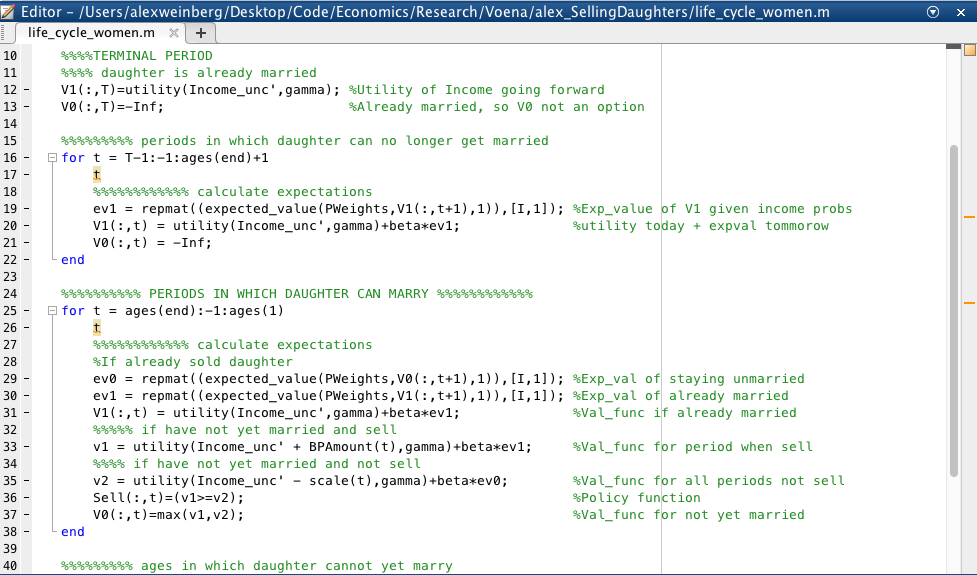
\includegraphics[width=1.0\linewidth]{code.png}
  \end{figure}
\end{frame}
%------------------------------------------------

\begin{frame}
\frametitle{My Work}

\begin{itemize}
\item More detailed subset of the paper in Tanzania
\item Finite horizon VFI, Optimal Stopping Probelm
\begin{enumerate}
  \item No savings decision
  \item When to sell your daughter?
\end{enumerate}
\item \textbf{Answer:} Using brideweath as consumption smoothing technique to smooth consumption when facing low-income shock.
\item \textbf{Policy Counterfactual:} If allow savings? Marriage age goes up because want to accrue more of the benefit daughter provides to home.
\end{itemize}

\end{frame}

%----------------------------------------------------------------------------------------

\end{document}
